% !TEX root = ../main.tex
\section{Evaluation of Graphical Password Schemes} \label{sec:evaluation}
	
  Authentication with text-based passwords are a common approach but it is well known that users often choose weaker passwords because of the limitations of recalling text-based passwords. Graphical passwords came as an alternative solution for overcoming the limitations of text-based passwords, and was inspired by researchers that showed that the graphical memory of humans is particularly well-suited to remember graphical information \cite{DeAngeli}. The problem with many graphical password schemes is that they often promise improved password memorability and thus usability, and at the same time improve the security \cite{Biddle}. The trade-off between usability and security is illustrated in Figure~\ref{fig:usabilitysecurity}. Because of the observed trade-off between usability and security, it is important to understand both aspects when reviewing the litterature of graphical passwords.

  	\begin{figure}[H]
  		\centering
  		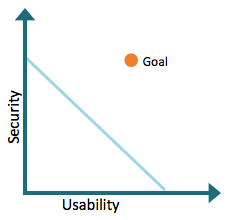
\includegraphics[width=0.40\textwidth]{pics/review/tradeoff.png}
  		\caption{Tradeoff between usability and security}
  		\label{fig:usabilitysecurity}
  	\end{figure}

	\clearpage
  \subsection{Usability and Memorability} \label{sec:usability}

    %INTRODUCTION
    An interesting question to be asked is what types of graphical password users find memorable. If the number of possible pictures in a graphical password scheme is large enough, and the diversity of the of picture based passwords can be captured, it seems reasonable to argue that memorable password space of a graphical password scheme will be higher than text-based password schemes. 

    %DEJA VU
    When the proposal for the graphical password scheme ``Deja Vu'' was proposed, the researchers conducted a user study showing that 90\% of all participants succeeded the authentication phase using the Deja Vu scheme, while 70\% succeeded in passing the correct password using text-based passwords and PIN codes \cite{DejaVu}. This is an example that users tend to have a higher success rate remembering graphical password over text-based passwords and PIN codes. 

    %DRAW A SECRET
    One of the first graphical password schemes, ``DAS'' \cite{Jermyn}, offers a theoretical space that are comparable with text-based passwords. Based on cognitive studies of visual information, Oorschot and Thorpe \cite{Thorpe1} investigated the memorable password space in the graphical password scheme DAS \cite{Jermyn}. They found that the memorable password space of the DAS were less or equal to the length of 8 on a 5$\times$5 grid. The results from research shows that users tend to draw symmetric images with few pen strokes, and often place their drawings in the center of the grid. The researchers behind ``Background Draw A Secret'' (BDAS) \cite{BDAS} tried to avoid users placing their drawings in a predictable way and therefore added an additional background image to avoid predictable behaviour. The attached background image resulted in a reduced amount of symmetry within the selected passwords, and supported the users to make longer passwords that were similarly memorable as for the ``DAS''.

    %STORY, FACE
    Davis \cite{Davis} did a comparison of the memorability between the graphical password scheme ``Face'' (a light version of the ``PassFaces'') and ``Story''. This results reported that users had more difficulty remembering Story password (success rate of 85\%), where most of the errors was introduced because they had to remember the correct sequence of the images.

    %ANDROID
    When looking at usability, we can evaluate the graphical layout of a graphical password scheme to see if the visual elements impacts the user's choice of passwords. Ullenbeck et al. \cite{Uellenbeck} looked at the Android Unlock patterns and investigated if a change in the graphical layout would impact the security. The Android Patten Lock is made on a 3$\times$3 grid of connected points. Instead, they rearranged the points in 4 different positions and analyzed patterns created by users. The results showed that they managed to double the password space by rearranging the points and reduce the biases that are found in the original position of the nodes. Unfortunately did they not only remove some of the bias from the original grid, but also introduced new ones. One of the rearrangements was a random approach. Unfortunately, this random arrangement of nodes looked like the mathematical ``delta'', so many people recognized this association element. The random arrangement scored the worst entropy since many of the users chose the same pattern. People are good at recognizing patterns and using association elements. It would not be surprisingly if users would find the same results in other rearrangements of the grid if it had a shape similar to other symbols or association elements.

    %PASSPOINT
    Wiedenbeck et al. \cite{Wiedenbeck1, Wiedenbeck2, Wiedenbeck3} conducted three lab-based user studies of the graphical password scheme ``PassPoint''. The results showed that the users needed an average time of 63 seconds in order to create their password, and an additional average time of 171 seconds in training time in order to remember the password. The login time took an average time of 9 and 19 seconds. This highlights important research on usability and memorability of a graphical password schemes. Some of the factors that make a password scheme to have high usability is deiced by average creation time, time to remember the password, as well as time used in the login phase. 

    %SUMMARY
    It remains still a problem that many of the published research on graphical passwords focusing on usability are performed with a pen and paper approach, raising a question about the validity of the results. One problem may be that many graphical passwords are not implemented, but rather theoretical and visual suggestions. It still a need for further research on graphical passwords in their actual intended environment of use.

    \todo{Legge til mere forskning på usability}

	\subsection{Security} \label{sec:security}

    In knowledge-based authentication, e.g. ``something you know'', we classify attacks into two general categories: guessing and capturing attacks. 
    In a guessing attack the attackers are needs to search through the entire password space, often referred to as a brute force attack. If the attacker have some knowledge of the user or the users password habits, the attacker would might be able to predict the users password based on the knowledge in order to avoid searching through the whole passwords space. This type of attack are often referred to as a dictionary attack. The success rate of the two mentioned types of guessing attacks are often associated with the entropy of the password scheme. A low entropy of a password scheme will result in less attempts in order to perform a successful guessing attack. When talking about capturing attacks, the attackers can directly obtain the passwords by observing the authentication process. One of the known capturing attacks on graphical passwords is shoulder surfing because of its graphical visualization.

    When a person select a password it is normal to choose a password that are connected to you as a person or to something you know. When using something connected to you or something you know in the process of creating a password it would probably be easier to remember because you already knows it. This is one of the core security issues when it comes to humans and passwords because the attackers utilize our predictable behavior. A password created using this predictable behavior are called a biased password. A bias can be explained as a prejudice in favor of or against one thing, person, or group compared with another, usually in a way that influence a person choice of action. 

    Jermyn et al. \cite{Jermyn} evaluated the security the graphical password scheme DAS. One of the statements is that the users do not use a uniform distribution of all possible passwords, using Klein's study \cite{UnixPasswords} as a argument. The fact that users do not pick passwords uniformly are no itself a sufficient statement to make a guessing attack successful. They try to cover the possibility of an attacker making a successful attack by making their scheme complex, and the results showed that the generated passwords were significantly harder to crack in practice than textual passwords. The problem with the conducted tests was that they used computer generated passwords that will not show real user-selected passwords. They did not analyze the security of the DAS including human factors and password biases that may influence the practical password space.

    Reviewing literature focusing on graphical password it is noticed that published research are lacking studies on users choices in graphical passwords. why do users select the passwords they do, and what strategy do they use in the creation process? Davis et al.\cite{Davis} evaluated the security of the graphical password scheme ``Passfaces''. They found that there was a bias introduced by peoples demographics and background, in other words biased by who you are. The users tended to choose faces that they liked (their own subjective meaning of beauty and attractiveness) and faces they could compare themselves to. The results showed that if you knew the gender and race of the user, you could perform a dictionary attack to guess user selected passwords. If the gender of the user was known as male, then 10\% of the passwords could easily be guessed on the first or second attempt. Similarly, if the race of the user was known to be Asian and his/her gender is known, then 10\% of the worst passwords could be guessed within the first six attempts. The results indicated that user-selected graphical passwords can be heavily biased, and concluded that Passfaces was insecure in particular due to the observations.

    Dirik et al. \cite{Dirik} conducted an experiment by modeling user choice in the graphical password scheme ``PassPoints''. The aim of this study was to test if it was possible to build a dictionary attack based on user's choice in clicking points. In this study, they predefined two different images with a different level of salient points. The results stated that they could recover 61\% of the user's passwords by searching through a smaller password space that was based on an analysis of collected click-points. The ``PassPoints'' scheme provides user-chosen password, but the aim of this study was to investigate if it was possible to predict users password using a dictionary attack. There was a slight difference in the two images picked by the researcher, where the image with less salient points was stated as insecure. Since the ``PassPoints'' scheme enables user-selected passwords, the security may rely on the selected image by the user, and not the actual scheme itself. The results of this research can not alone state that the ``PassPoints'' scheme is insecure. It rather highlights the importance of considering the human factors in security because it may influence the overall security of a graphical password scheme. The same year another research group published \cite{Thorpe2} results on security of the ``Passpoints'', but using different approaches. They conducted a user study to test if it was possible to make an offline attack as well as using an image-processing tool for simulating an offline attack on the same images that were used in the user studies. They provided empirical evidence that attractive points, e.g. hot-spots, do exist in images. The results from the most efficient attack were generated by harvesting passwords from users to attack other targets. The probability of the guessing attack showed that 36\% of the passwords selected by users could be guessed within $2^{31}$ guesses and 12\% within $2^{16}$ guesses. The results from the offline attack using image-processing were slightly less efficient, but they still managed to prove that an offline attack is possible to use on graphical passwords.

    In one of the first large-scale studies on the Android Pattern Lock \cite{Uellenbeck} it was stated that the entropy of patterns is lower than its theoretical entropy. The results of the study indicated that the security offered is less than the security of only three digits randomly assigned PIN for guessing 20\% of all passwords. In the same research, they made a Markov model based on collected passwords from users categorized as offensive and defensive patterns in their user study. The results showed that it was possible to guess user's choice in patterns. Within ten guesses they could guess approximately 4\% of pattern in the category defensive patterns and approximately 7\% of the defensive patterns. When increasing the number of guesses to 30 attempts, they managed to guess approximately 9\% of the defensive patterns and approximately 19\% of the offensive patterns. If we look further into the Android Unlock Pattern, it have nearly 400.000 possible patterns and are from a theoretical point of view stronger than a 5-digit randomly assigned PIN. The researchers evaluation of user chosen patterns shows that they only have an estimated entropy slightly lower than a 3-digit randomly assigned PINs. Another interesting result is the memorable password space used, where about 10\% of all users use less than 190 patterns, while less than 300 patterns capture around 50\% of the whole test population. This shows that an empirical password space are not a representative number when quantifying the security of a password. We should rather look at the memorable password space, e.g. password that are used and memorized by users.

    Since psychological studies have recognized that the human brain have a superior memory for recognizing and recalling visual information, it support the statement that users are able to remember more complicated graphical password form a larger password space than a alphanumeric password. Logically the attacker then has to build a bigger and more complex dictionary, thus spend more time to achieve the same success rate as for textual passwords. A clever attacker would narrow down the password space and prioritize guesses to pictures that people are likely to choose. The images that are selected are liable to be the images that users are likely to recall. In order to understand how an attacker might take advantage of human password choices, psychological studies on humans visual memory are crucial to comprehend. 
